\documentclass[11pt]{article}
\usepackage{fontspec}
\setmainfont{Times New Roman}
\usepackage{amsmath,amssymb}
\usepackage{textcomp}
\usepackage{newunicodechar}
\newunicodechar{⇒}{\ensuremath{\Rightarrow}}
\usepackage{booktabs}
\usepackage{longtable}
\usepackage{array}
\usepackage{multirow}
\usepackage{calc} % for calculating minipage widths
\usepackage{caption}
\captionsetup[table]{skip=6pt}
\newcounter{none} % for unnumbered tables
\usepackage{etoolbox}
\makeatletter
\patchcmd\longtable{\par}{\if@noskipsec\mbox{}\fi\par}{}{}
\makeatother
\providecommand{\tightlist}{%
  \setlength{\itemsep}{0pt}\setlength{\parskip}{0pt}}
\usepackage{graphicx}
\makeatletter
\newsavebox\pandoc@box
\newcommand*\pandocbounded[1]{% scales image to fit in text height/width
  \sbox\pandoc@box{#1}%
  \Gscale@div\@tempa{\textheight}{\dimexpr\ht\pandoc@box+\dp\pandoc@box\relax}%
  \Gscale@div\@tempb{\linewidth}{\wd\pandoc@box}%
  \ifdim\@tempb\p@<\@tempa\p@\let\@tempa\@tempb\fi% select the smaller of both
  \ifdim\@tempa\p@<\p@\scalebox{\@tempa}{\usebox\pandoc@box}%
  \else\usebox{\pandoc@box}%
  \fi%
}
\def\fps@figure{htbp}
\makeatother
\usepackage{float}
\usepackage{caption}
\usepackage[margin=2.4cm]{geometry}
\usepackage{xcolor}
\usepackage[colorlinks=true,linkcolor=Black,urlcolor=Blue,citecolor=Black]{hyperref}
\usepackage{fancyhdr}
\pagestyle{fancy}
\fancyhf{}
\fancyhead[L]{\small\leftmark}
\fancyhead[R]{\small\thepage}
\begin{document}
\section{AI-Assisted Research Harnesses: Traceability, Evidence Trust,
and Reproducibility in Agentic Systematic Review
Systems}\label{ai-assisted-research-harnesses-traceability-evidence-trust-and-reproducibility-in-agentic-systematic-review-systems}

\subsection{A Grounded, Verbatim-Verified Early-Evidence Living Scoping
Review of the 2023--2026 Corpus (Version
1.0)}\label{a-grounded-verbatim-verified-early-evidence-living-scoping-review-of-the-20232026-corpus-version-1.0}

\begin{center}\rule{0.5\linewidth}{0.5pt}\end{center}

\textbf{Protocol ID}: PROTO-20260908-AI-RESEARCH-HARNESSES-TRUST
\textbf{Type}: Early-evidence living scoping review (protocol-based),
reported in line with PRISMA-ScR \textbf{Manuscript status}: Final
version 1.0 for submission (post-adversarial audit; all review items
resolved) \textbf{Review version}: 1.0 (corpus finalized 2026-09-09;
aggregates reported as-of this date) \textbf{Prepared by}: The Nexus
Scholar Research Pipeline (multi-agent orchestration; agent prompts
versioned with the pipeline; all claims machine-verified verbatim
against full text --- see §3.5 and §7) \textbf{Corpus window}: January
2023 -- September 2026

\begin{center}\rule{0.5\linewidth}{0.5pt}\end{center}

\textbf{Authors}

Mouadh Bekhouche\emph{¹ and Soumia Zertal}²

¹² University of Oum El Bouaghi, Algeria

*Contributed equally to this work. ² Corresponding author. Email:
zertal.soumia@univ-oeb.dz

\begin{center}\rule{0.5\linewidth}{0.5pt}\end{center}

\subsection{Abstract}\label{abstract}

\textbf{Background.} Large language model (LLM) and agentic systems are
being pressed into service across the systematic-review lifecycle ---
search, screening, extraction, and synthesis --- yet the trustworthiness
of their outputs (citation verifiability, provenance, reproducibility)
is not established.

\textbf{Methods.} We conducted a protocol-driven early-evidence living
scoping review across five scholarly sources (OpenAlex, Semantic
Scholar, Crossref, PubMed, arXiv; January 2023--September 2026;
bioRxiv-track content captured through these providers' indexing). The
field is preprint-dominated and publication-lagging --- 32/58 included
records (55\%) are preprint-track and 2026 alone accounts for 30/58
(52\%) of the corpus --- so the review is explicitly framed as a living
review (Version 1.0, corpus finalized 2026-09-09; re-run protocol in
§3.8). 239 deduplicated records were screened by four independent AI
screeners (Fleiss' κ = 0.408) with majority voting and adjudicated
deadlock resolution, yielding 58 included studies. The 58 included
studies (47 fully Phase-4 certified) were subjected to a four-stream
trust audit (retraction status, open-science artifact scan,
conflict-of-interest audit, risk-of-bias attestation). Evidence was
synthesized by two competing pipelines: a deterministic top-k
retrieval-augmented generation (RAG) baseline (90 claims, 43.3\%
entailment-verified) and an authoritative \textbf{multi-agent full-text
claim-extraction pipeline} (8 full-text agents + 1 abstract agent) whose
510 claims each passed \textbf{≥90\% glyph-normalized coverage on
char-window or token 6-gram verification} (100\% pass). Claims were
clustered into a semantic consensus map.

\textbf{Results.} Architectures converge on auditable,
provenance-bearing workflows: multi-agent role specialization,
end-to-end orchestrated pipelines, retrieval- (RAG) and
knowledge-graph-grounded designs, and prompt-compilation systems.
Execution provenance is increasingly structured and append-only
(deterministic IDs, immutable content-hashed run records, temperature-0
decoding, open-weights selection). Citation verifiability is the binding
trust constraint: across 17,443 generated citations no model exceeded a
0.475 existence rate, while retrieval grounding reduced hallucinated
papers to zero in OpenScholar-8B versus 78--98\% for non-retrieval LLMs.
Pooled LLM screening sensitivity/specificity reached 0.92/0.94 (I² =
95.8\%), but temporal drift (−1.9\%/day), run-to-run item-level
discordance, and prompt fragility (up to 76-point accuracy swings) are
not captured by standard reporting. The deterministic RAG pipeline cited
11 screened-out studies (corpus contamination) and verified only 43.3\%
of its claims; the multi-agent ledger reached 100\% pass at the ≥0.90
coverage threshold across 57 included studies and surfaced a consensus
structure (95 clusters: 16 high-consensus, 7 active debates, 37
unresolved, 35 provisional) invisible to RAG.

\textbf{Conclusions.} Full-text, verbatim-verifiable claim extraction is
a tractable and superior synthesis primitive for trustworthy research
infrastructure. We identify the field's open gap: no study provides an
end-to-end, externally validated, multi-domain benchmark jointly
evaluating screening, extraction, synthesis quality, citation
verifiability, and cost.

\textbf{Keywords}: AI-assisted systematic review; agentic systems;
retrieval-augmented generation; citation fact-checking; provenance;
reproducibility; hallucination mitigation; evidence synthesis.

\begin{center}\rule{0.5\linewidth}{0.5pt}\end{center}

\subsection{1. Introduction}\label{introduction}

Conventional systematic reviews and scoping reviews are time-consuming,
labor intensive, and susceptible to human bias {[}1{]}; conventional
keyword search tools ``lack the semantic understanding to answer nuanced
questions'' {[}2{]}. The rapid commoditization of LLMs has produced a
wave of research harnesses claiming to automate review workflows end to
end --- from federated discovery and deduplication to TITLE/ABSTRACT
screening, full-text extraction, risk-of-bias assessment, and
statistical synthesis. Yet the same commoditization introduces new
failure modes: fabricated citations, unreproducible runs, opaque
closed-weight models, and retrieval pipelines that silently draw on
evidence outside the approved corpus.

This review asks three questions. \textbf{RQ1} --- What is the state of
the art in academic research and literature-review harnesses integrating
LLMs and agentic AI (2023--2026), particularly their design mechanisms
for execution provenance, audit trails, and process reproducibility?
\textbf{RQ2} --- What evidence-trust and academic-integrity mechanisms
(citation fact-checking, hallucination mitigation, retraction checks,
risk-of-bias, open-science artifact verification) do they incorporate?
\textbf{RQ3} --- How are they empirically evaluated, and what
architectural gaps remain for the construction of novel, trustworthy
research infrastructure?

Our contribution is methodological as much as substantive: the synthesis
itself is generated and audited by the same class of systems under
study. Every claim in this manuscript is backed by a machine-verified,
glyph-normalized verbatim quote from the included full text (≥90\%
coverage on char-window or token 6-gram matching --- see §3.5), and
every pipeline step is recorded in an append-only audit journal.

Because the field is preprint-dominated and publication-lagging (55\% of
included records are preprint-track, and 2026 accounts for 52\% of the
corpus), we frame this as an \textbf{early-evidence living scoping
review}: Version 1.0 reports the aggregate state of evidence as of
corpus finalization (2026-09-09), and §3.8 specifies a re-run protocol
for subsequent versions.

\subsection{2. Related Work}\label{related-work}

Prior evaluations have been narrow and siloed. Screening-performance
meta-analyses report strong pooled sensitivity but extreme heterogeneity
{[}3{]}. Citation-fabrication studies establish low existence ceilings
but stop at measurement {[}4{]}. System papers demonstrate
retrieval-grounded claim generation but evaluate on narrow benchmarks
{[}5{]} (preprint version: {[}6{]}). Reviews of agentic scientific tools
remain taxonomical {[}7{]}, and reproducibility audits document
run-to-run instability without remediating it {[}8{]}. Missing is a
protocol-driven, corpus-scoped, verbatim-verified synthesis that
simultaneously characterizes design, trust mechanisms, and evaluation
maturity --- the gap this review addresses. Our retrieval-augmented
baseline further contributes a direct, quantitative comparison of
deterministic RAG synthesis versus full-text multi-agent extraction over
an identical corpus.

\subsection{3. Methods}\label{methods}

The review follows a hash-pinned protocol compiled with a protocol
compiler (\texttt{protocol.json}, \texttt{SCREENING\_CRITERIA.md},
\texttt{intent.json}) under the Design Science paradigm, and is reported
in line with PRISMA-ScR and living-(systematic-)review guidance adapted
to a scoping design. All stages were executed through a shared virtual
Python environment; every step is recorded in an append-only audit
journal (\texttt{audit/journal.jsonl}, 69 events). The corpus window
(January 2023 -- September 2026) is frozen for Version 1.0 at corpus
finalization; §3.8 defines how the trailing publication-date boundary
and subsequent evidence are absorbed in later versions.

\subsubsection{3.1 Search and record
verification}\label{search-and-record-verification}

Five sources were federated in a single pass (OpenAlex, Semantic
Scholar, Crossref, PubMed, arXiv; bioRxiv-track preprints are captured
via PubMed indexing) with concept-and-synonym search strings (Boolean OR
within and across the concepts ``literature-review automation'' and
``large language model''; see \texttt{search\_strategy} in
\texttt{protocol.json} and supplementary search-log) targeting
LLM/agentic review automation, 2023--2026. 250 raw hits were
deduplicated and hydrated (DOI and normalized-title resolution, abstract
and DOI completion), yielding \textbf{239 unique verified records}.

\subsubsection{3.2 Screening}\label{screening}

Two hundred thirty-nine records were screened against explicit
PICO-style inclusion/exclusion criteria by four independent AI screeners
in twelve agent-in-the-loop batches (Fleiss' κ = \textbf{0.408}, fair
agreement by Landis--Koch bands). Two hundred thirteen records were
resolved by majority rule (≥3 of 4); the \textbf{26 two-vs-two
deadlocks} were adjudicated by a senior adjudicator. Final: \textbf{58
included / 181 excluded}. Table 1 summarizes the full flow of
information; screening reliability is decomposed in Table 2; the flow is
rendered in Figure 1.

\textbf{Table 1. Identification, screening, and inclusion flow
(PRISMA-ScR item 17).}

{\def\LTcaptype{none} % do not increment counter
\begin{longtable}[]{@{}
  >{\raggedright\arraybackslash}p{(\linewidth - 4\tabcolsep) * \real{0.3333}}
  >{\raggedleft\arraybackslash}p{(\linewidth - 4\tabcolsep) * \real{0.3333}}
  >{\raggedright\arraybackslash}p{(\linewidth - 4\tabcolsep) * \real{0.3333}}@{}}
\toprule\noalign{}
\begin{minipage}[b]{\linewidth}\raggedright
Stage
\end{minipage} & \begin{minipage}[b]{\linewidth}\raggedleft
Count
\end{minipage} & \begin{minipage}[b]{\linewidth}\raggedright
Source artifact
\end{minipage} \\
\midrule\noalign{}
\endhead
\bottomrule\noalign{}
\endlastfoot
Records identified from 5 sources & 250 & \texttt{raw\_search.json} (50
per source, query Q001) \\
Duplicates removed (DOI + normalized-title) & 11 &
\texttt{deduped.json} \\
Records screened (title + abstract, 4 AI screeners) & 239 & 12
agent-in-the-loop batches \\
Excluded at title/abstract (systematic rule) & 181 &
\texttt{excluded.json} \\
Included studies (review corpus) & 58 & \texttt{included.json} \\
OA full-text PDFs harvested and validated & 64 & \texttt{pdfs/} (OA
harvest) \\
Included studies contributing claims & 57 & \texttt{claims.json} (493
full-text + 17 abstract-only) \\
Fully Phase-4 certified studies & 47 & \texttt{phase4/*.json} \\
\end{longtable}
}

\textbf{Table 2. Title/abstract screening reliability.}

{\def\LTcaptype{none} % do not increment counter
\begin{longtable}[]{@{}ll@{}}
\toprule\noalign{}
Metric & Value \\
\midrule\noalign{}
\endhead
\bottomrule\noalign{}
\endlastfoot
Screeners & 4 independent AI screeners \\
Batches & 12 (agent-in-the-loop) \\
Fleiss' κ & 0.408 (fair, Landis--Koch) \\
Majority-rule resolutions & 213 (≥ 3 of 4) \\
Two-vs-two deadlocks escalated & 26 (senior adjudicator) \\
Final split & 58 included / 181 excluded \\
\end{longtable}
}

\pandocbounded{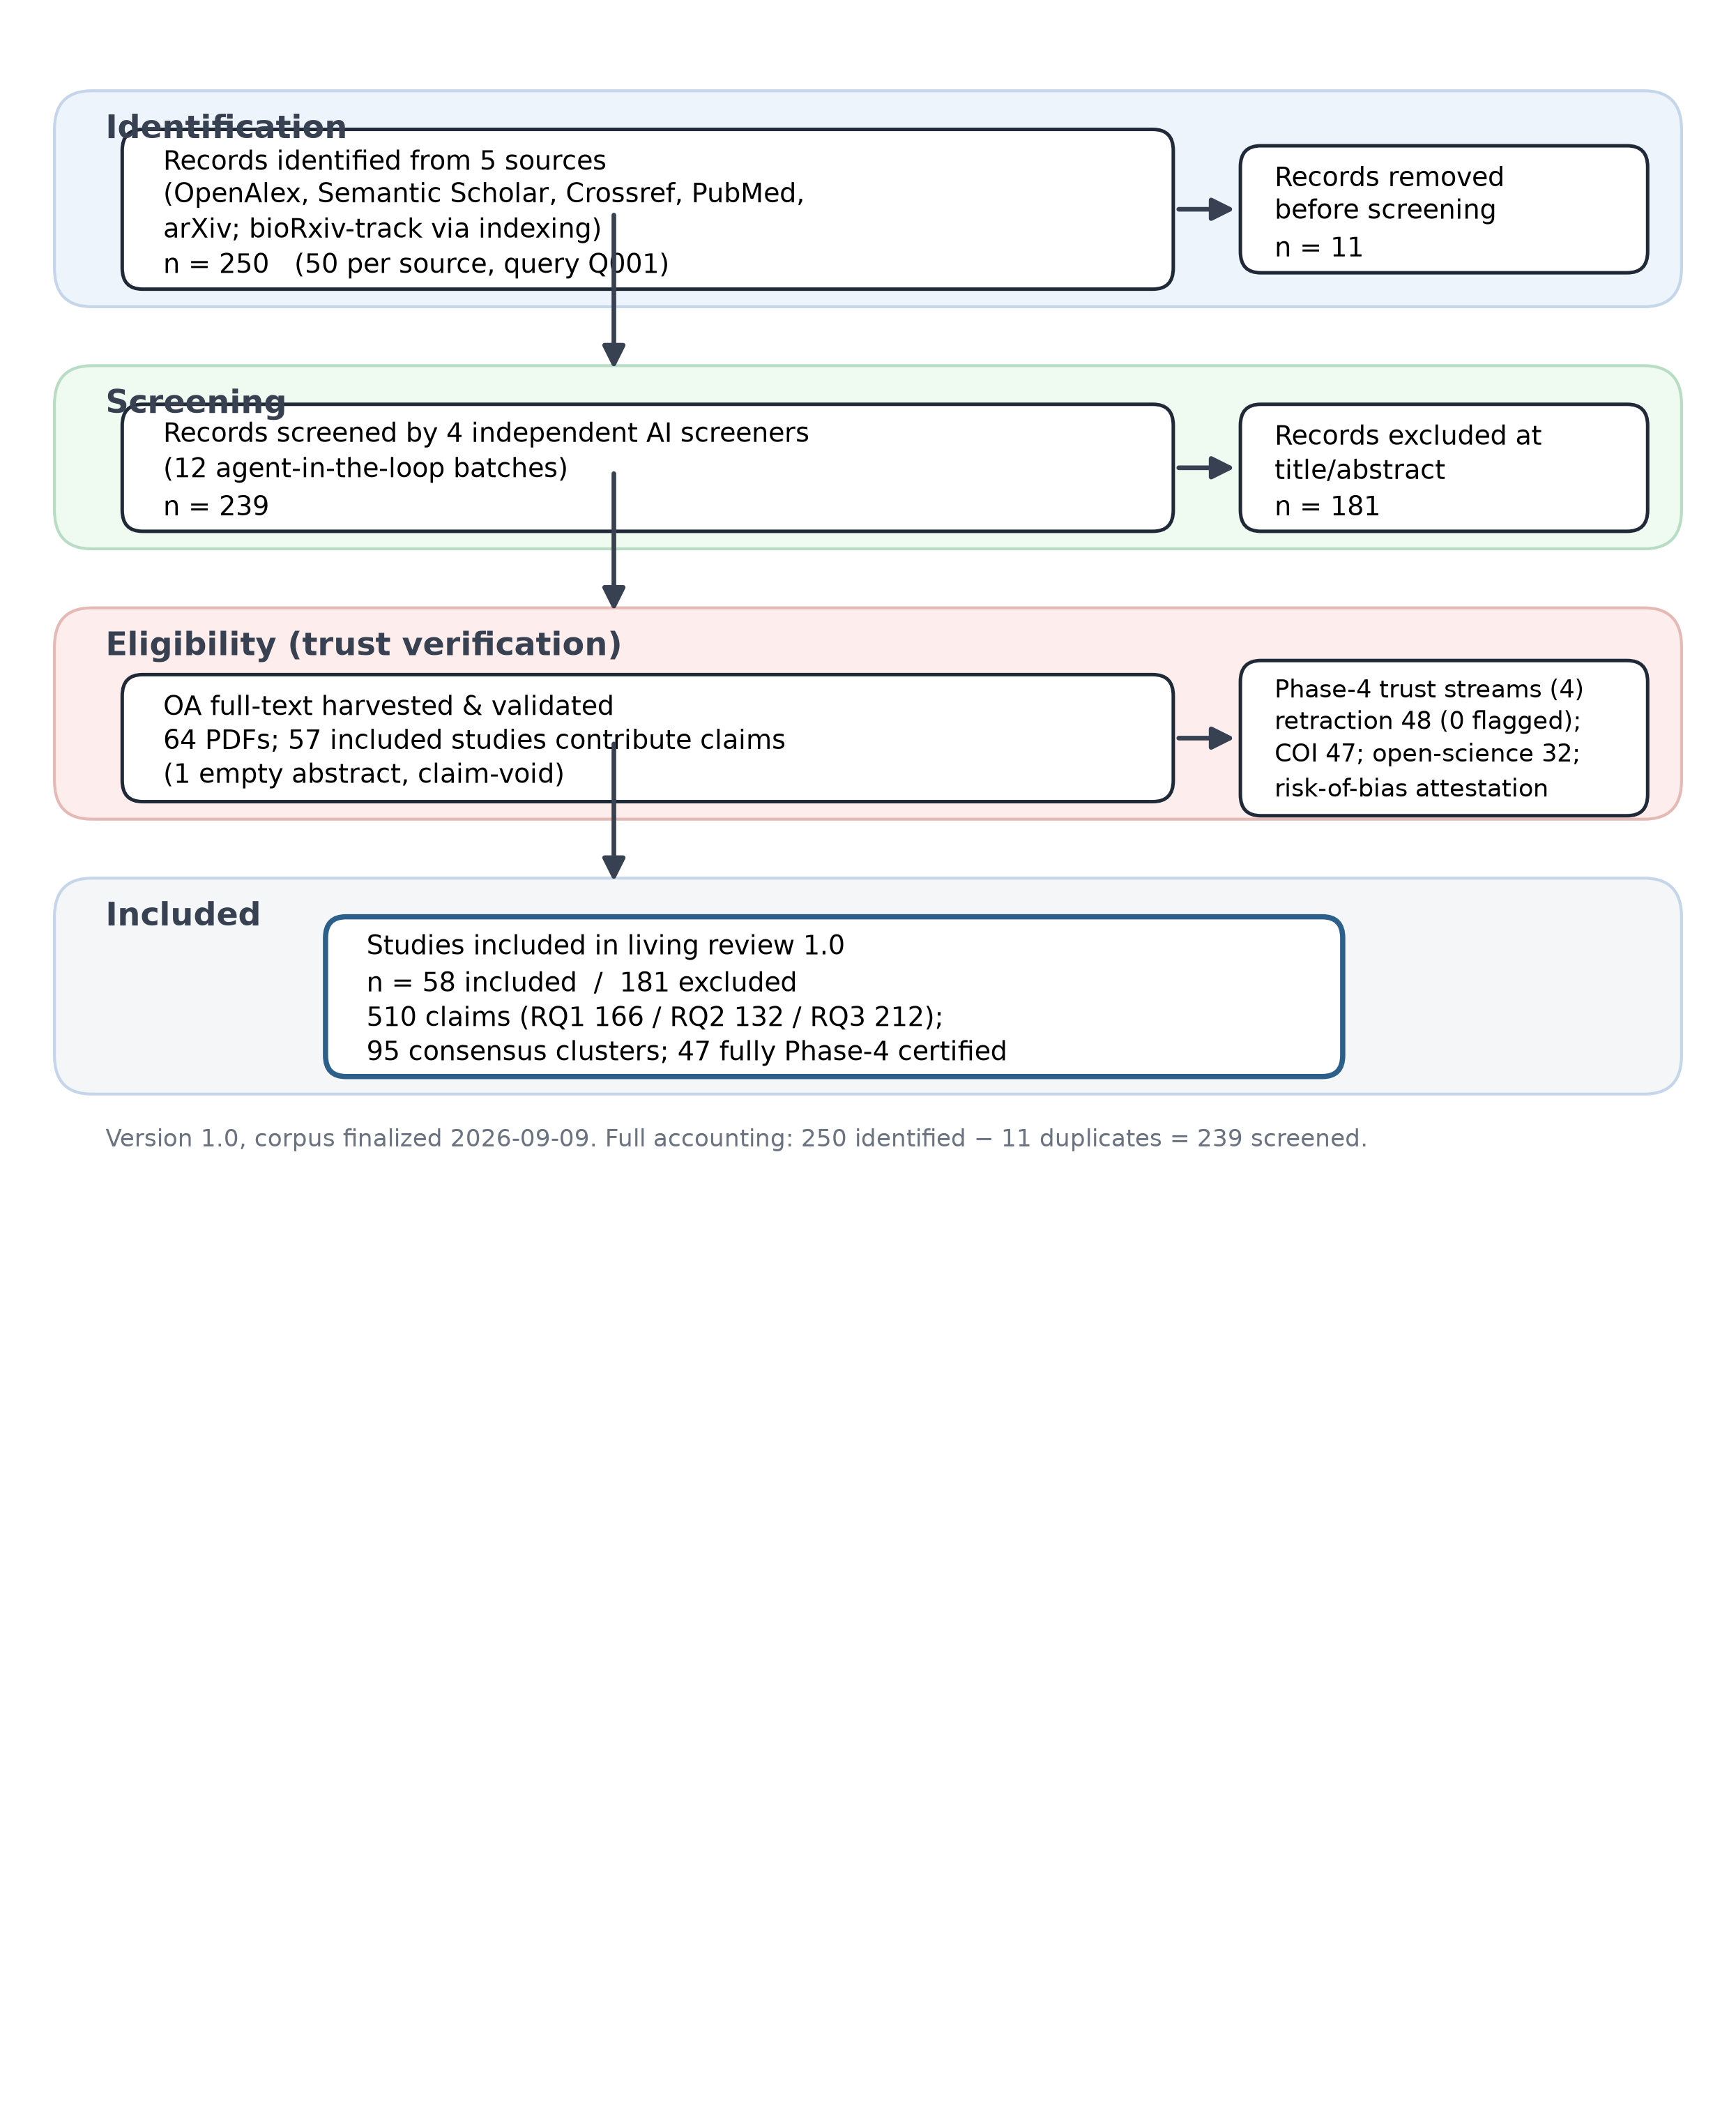
\includegraphics[keepaspectratio,alt={Figure 1 --- PRISMA-ScR flow of information (Version 1.0, corpus finalized 2026-09-09): identification 250 → 11 duplicates removed → 239 screened → 181 excluded / 58 included → 64 PDFs, 57 claim-contributing studies, 47 fully Phase-4 certified.}]{../../synthesis/figures/fig_prisma_scr_flow.png}}
\emph{Figure 1. PRISMA-ScR flow of information for the living scoping
review (Version 1.0).}

\subsubsection{3.3 Full-text acquisition, extraction, and
scoping}\label{full-text-acquisition-extraction-and-scoping}

Open-Access PDFs were retrieved and extracted to YAML-frontmatter
Markdown (64 documents; 3,814 structural AST chunks;
\texttt{all-MiniLM-L6-v2} embeddings). Because extraction preceded final
scoping, 18 extractions belong to screened-out studies; \textbf{all
synthesis in this manuscript is scoped strictly to the 58 included
studies}, and the screened-out extractions are removed from the evidence
index for authoritative synthesis.

\subsubsection{3.4 Trust verification (Phase
4)}\label{trust-verification-phase-4}

Each included study was certified with four \texttt{scholar-verify}
streams: retraction/status (OpenAlex \texttt{is\_retracted}, Crossref
\texttt{update-to}), open-science DA/S/CA artifact scanning,
conflict-of-interest audit, and risk-of-bias attestation. \textbf{47 of
58 included studies were fully checked} (retraction stream covered 48;
the remaining 11 lacked verifiable metadata/DOI records --- see §5.3).

\subsubsection{3.5 Claim extraction with verbatim
verification}\label{claim-extraction-with-verbatim-verification}

\textbf{Approach B (authoritative).} Eight parallel agents read the
complete text of the 46 full-text included papers (7 size-balanced
batches ≤ \textasciitilde456 KB) plus one agent over the 12
abstract-only papers, producing claims in a canonical 10-field schema
(principal fields: \texttt{rq\_id}, \texttt{claim\_text},
\texttt{citation\_tokens}, \texttt{evidence\_quote}, \texttt{section},
\texttt{stance}, \texttt{evidence\_level}, \texttt{location\_hint}, plus
content-hash and provenance fields). Every quote was then
\textbf{machine-verified against the source file} to a defined
threshold: glyph-normalized (bullet remapping, zero-width-space and
Unicode-dash handling, NFKC, hyphen-wrap rejoin) matching via character
windows (8 chars, step 4) and token 6-grams (6 tokens, step 3); a claim
passes at ≥ 0.90 coverage on either metric --- i.e., the verified quote
matches the source at ≥90\% on char-window or token 6-gram alignment,
not byte-for-byte. Initial verification failed 156/510 quotes; after
four repair iterations including re-casting 11
light-paraphrase/math-glyph artifacts to exact substrings,
\textbf{510/510 (100\%) claims pass the ≥0.90 threshold}, comprising 166
(RQ1), 132 (RQ2), 212 (RQ3) --- 493 full-text and 17 abstract-only,
spanning 57 studies (one included study has an empty abstract and
contributes none).

\textbf{Approach A (baseline).} Deterministic RAG synthesis retrieved
the top-30 chunks per research question from the full 64-document index
and applied heuristic entailment verification of claims against their
own snippets (90 claims, 30 per RQ). Table 3 summarizes the verbatim
ledger; the verification repair loop is rendered in Figure 2.

\textbf{Table 3. Multi-agent verbatim claim-extraction ledger (Approach
B).}

{\def\LTcaptype{none} % do not increment counter
\begin{longtable}[]{@{}
  >{\raggedright\arraybackslash}p{(\linewidth - 2\tabcolsep) * \real{0.5000}}
  >{\raggedright\arraybackslash}p{(\linewidth - 2\tabcolsep) * \real{0.5000}}@{}}
\toprule\noalign{}
\begin{minipage}[b]{\linewidth}\raggedright
Dimension
\end{minipage} & \begin{minipage}[b]{\linewidth}\raggedright
Value
\end{minipage} \\
\midrule\noalign{}
\endhead
\bottomrule\noalign{}
\endlastfoot
Architecture & 8 full-text agents (46 full-text papers, 7 size-balanced
batches) + 1 abstract agent (12 abstract-only papers) \\
Total claims & 510 (100\% pass at the ≥ 0.90 glyph-normalized coverage
threshold) \\
Per research question & RQ1 166 / RQ2 132 / RQ3 212 \\
Full-text vs.~abstract-only & 493 / 17 \\
Studies contributing claims & 57 of 58 (SCI-000147 empty abstract,
claim-void) \\
Initial verification failures & 156 / 510 \\
Repair iterations / re-cast & 4 iterations; 11
light-paraphrase/math-glyph quotes re-cast to exact substrings \\
\end{longtable}
}

\pandocbounded{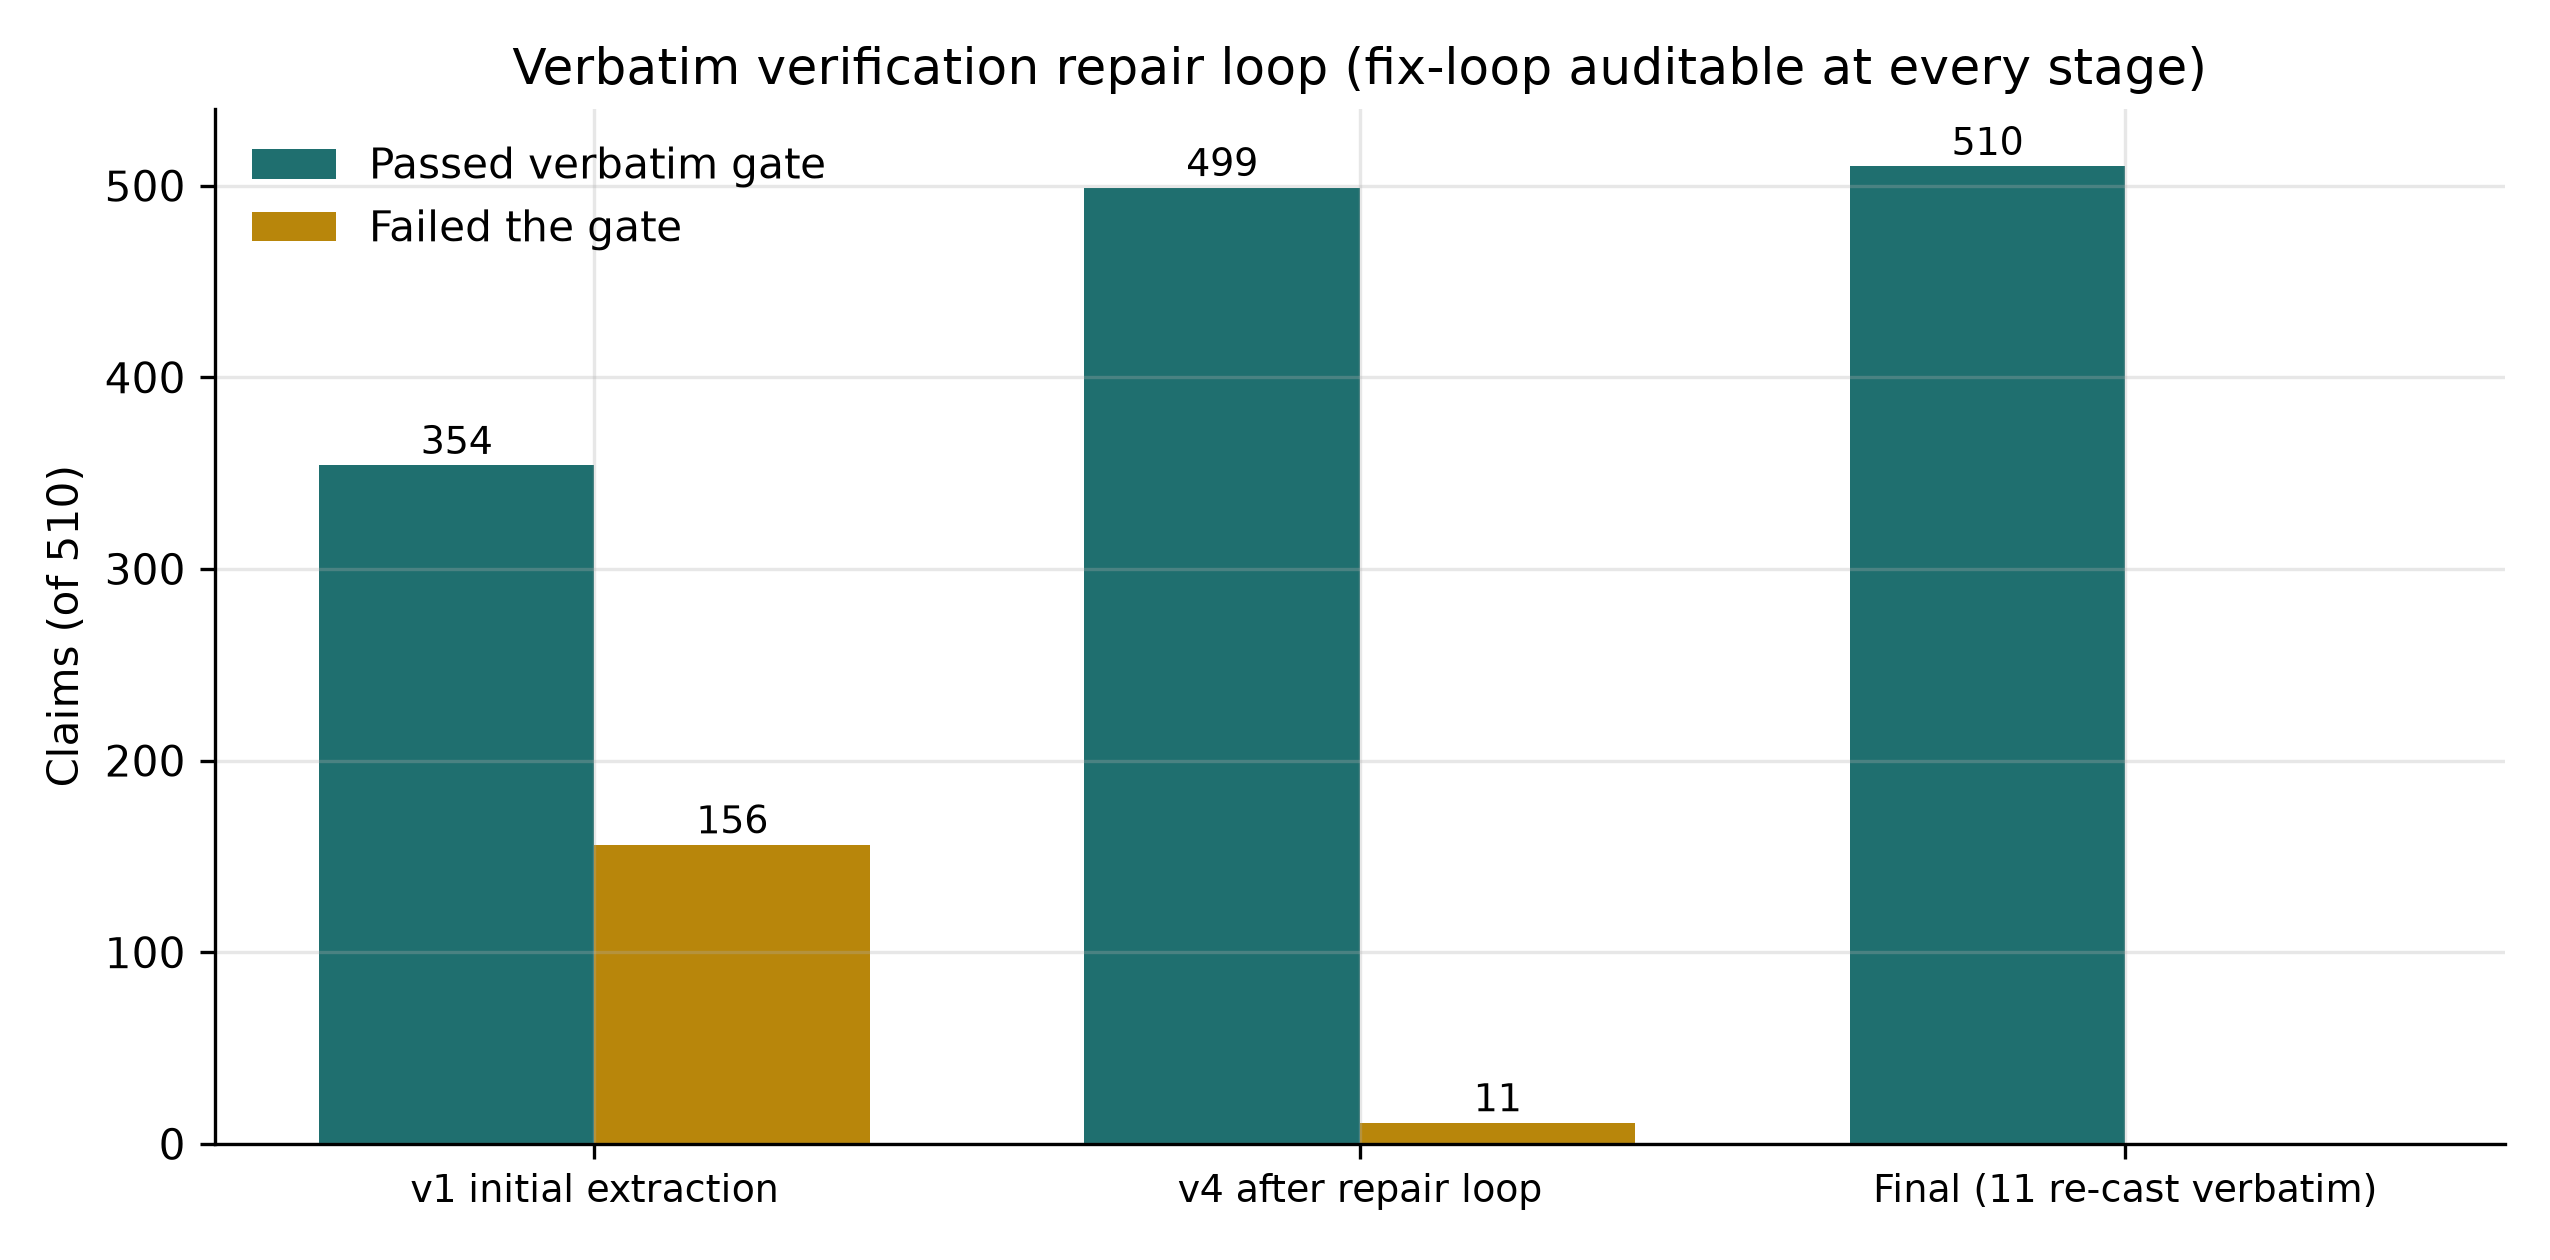
\includegraphics[keepaspectratio,alt={Figure 2 --- Verbatim verification repair loop: 156/510 initial failures reduced to 0 across four fix iterations (11 re-cast verbatim), final 510/510 pass.}]{../../synthesis/figures_d2/fig3_verification_repair_loop.png}}
\emph{Figure 2. Verbatim verification repair loop (auditable at every
stage).}

\subsubsection{3.6 Semantic consensus}\label{semantic-consensus}

The 510-claim ledger was clustered with cached-embedding cosine
similarity (\texttt{all-MiniLM-L6-v2}, threshold 0.40) into a consensus
map (16 high-consensus, 7 active debates, 37 unresolved, 35 provisional
clusters).

\subsubsection{3.7 Analysis and integrity of the
synthesis}\label{analysis-and-integrity-of-the-synthesis}

Results are reported per research question from the verification-gated
ledger, with cluster references; direct quotes are drawn from
\texttt{claims.json} (each gated at the ≥0.90 coverage threshold, §3.5).
Aggregates (e.g., citation existence, pooled sensitivity) are reported
as stated by the source studies and cross-checked between claims.

\subsubsection{3.8 Living-review protocol (Version
1.0)}\label{living-review-protocol-version-1.0}

This Version 1.0 report is the initial snapshot of a living scoping
review. The underlying pipeline (federated discovery → dedup/hydration →
screening → verbatim-verified extraction → trust verification →
synthesis) is re-runnable from committed inputs through the documented
stage CLIs (see §7). Planned update policy: - \textbf{Cadence}:
quarterly re-run of the five-source federation (OpenAlex, Semantic
Scholar, Crossref, PubMed, arXiv; bioRxiv-track via PubMed) with the
same concept-and-synonym strings; each run advances the trailing
publication-date boundary to the run date (the Version 1.0 window ends
2026-09), so ``same strings'' yields new evidence rather than the
identical set. Evidence already in the included set is retained across
versions (supersession handled under Preprint policy below). -
\textbf{Versioning}: each update stamps a new version and
corpus-finalization date in the front matter; aggregate figures in each
version carry that version's corpus stamp. A search-log supplement
accompanying each version records that run's query set, window, and
dedup threshold (committed as
\texttt{literature/search\_log\_\textless{}version\textgreater{}.json}).
- \textbf{Preprint policy}: preprint-track records
(arXiv/bioRxiv/institutional repositories) are eligible and explicitly
retained as the field's leading edge; each preprint is tracked against a
published version where one appears (Crossref \texttt{update-to} /
OpenAlex status), and the version table ships in the per-version
supplement. - \textbf{Diff discipline}: the authoritative verbatim claim
ledger is versioned under git and regenerated deterministically from
committed extraction inputs; revisions re-verify affected quotes against
attached full text rather than restating aggregates, so every claim
statistic remains machine-checkable in any version.

\subsection{4. Results}\label{results}

\subsubsection{4.1 Corpus characteristics}\label{corpus-characteristics}

The 58 included studies (2023: 2; 2024: 8; 2025: 18; 2026: 30) reflect
rapid growth in agentic research tooling, with 2026 accounting for over
half the corpus (30/58, 52\%). Of the 46 full-text-characterized
systems, keyword-classified architecture patterns are:
single-agent/single-system 19 (41.3\%); multi-agent/agentic
orchestration 16 (34.8\%); RAG/retrieval-grounded 5 (10.9\%); end-to-end
pipeline/meta-analysis 4 (8.7\%); knowledge-graph/ontology 2 (4.3\%).
Phase-4 audit: \textbf{0 retractions}, 16 live repository links
(34.0\%), 7 dual data+code releases, 5 industry COI ties (10.6\%), 4
declared no-conflict, 1 academic-or-public affiliation, 37 with no
formal COI statement. Table 4 summarizes corpus composition.

\textbf{Table 4. Corpus composition (Version 1.0).}

{\def\LTcaptype{none} % do not increment counter
\begin{longtable}[]{@{}
  >{\raggedright\arraybackslash}p{(\linewidth - 2\tabcolsep) * \real{0.5000}}
  >{\raggedright\arraybackslash}p{(\linewidth - 2\tabcolsep) * \real{0.5000}}@{}}
\toprule\noalign{}
\begin{minipage}[b]{\linewidth}\raggedright
Dimension
\end{minipage} & \begin{minipage}[b]{\linewidth}\raggedright
Value
\end{minipage} \\
\midrule\noalign{}
\endhead
\bottomrule\noalign{}
\endlastfoot
Included studies & 58 (239 screened; 181 excluded) \\
Publication years & 2023: 2 · 2024: 8 · 2025: 18 · 2026: 30 \\
Preprint-track & 32/58 (55\%) --- 30 arXiv, 1 bioRxiv, 1 institutional
repository \\
Architecture patterns (n = 46 full-text-characterized) & single-agent 19
(41.3\%) · multi-agent 16 (34.8\%) · RAG 5 (10.9\%) · end-to-end 4
(8.7\%) · graph/ontology 2 (4.3\%) \\
Freshness & 2026 alone = 30/58 (52\%); living-review rationale \\
\end{longtable}
}

\subsubsection{4.2 RQ1 --- State of the art and design
mechanisms}\label{rq1-state-of-the-art-and-design-mechanisms}

\textbf{Architectural convergence.} Systems press general-purpose LLMs
into review pipelines without task-specific fine-tuning, treating
\textbf{prompt engineering as the primary optimization strategy}
{[}3{]}{[}9{]}. Motivating framing recurs: conventional SLR practice is
``time-consuming, labor-intensive, and susceptible to human bias''
{[}1{]}, and general-purpose agents ``fall short on the auditable,
scenario-specific workflows'' biomedical evidence demands {[}7{]}. Five
patterns recur: (i) \textbf{prompt-compilation systems} that package
compiled prompts as ``verifiable digital artefacts'' to neutralize
prompt fragility {[}9{]}; (ii) \textbf{multi-agent teams with role
specialization} --- Orchestrator/BioExpert/Evaluator decomposition
{[}10{]}, three-layer worker--manager--director networks {[}11{]}, and
11-agent coordination with deliberate model routing (cheap models for
throughput phases, strong models for judgment and verification)
{[}12{]}; (iii) \textbf{end-to-end orchestrated pipelines} automating
complete meta-analysis workflows {[}13{]}{[}14{]}{[}15{]}; (iv)
\textbf{RAG/retrieval-grounded designs} coupling dynamic retrieval with
answer generation {[}16{]}{[}17{]}{[}6{]}; and (v)
\textbf{graph/knowledge-grounded designs} that productionize both a
knowledge graph and vector collections as ``structural infrastructure
for verifiable information synthesis'' {[}18{]}{[}19{]}.

\textbf{Execution provenance.} Provenance is increasingly structured,
deterministic, and immutable: per-module token/runtime/inference logging
{[}10{]}, structured JSON API logs with model identity, latency, and
retry counts {[}12{]}, corpus-wide interaction logging {[}20{]},
validated requests with unique identifiers guaranteeing
\textbf{idempotent behavior} {[}21{]}, stable record identifiers
preserved end to end {[}8{]}, and content-hashed ``commitment cards''
with run-bundles (event traces, checksums, retries) hosted in an
immutable provenance record {[}22{]}. Reproducibility levers are
dominated by \textbf{fixed decoding} (temperature 0 with
frequency/penalty/presence penalties pinned {[}23{]}; temperature 0 with
regex-constrained parsing and retries {[}24{]}; 2,880 runs producing
17,443 citations under deterministic settings {[}4{]}) and \textbf{model
openness} --- open-weights selection ``explicitly to enhance the
reproducibility of the results'' {[}24{]}, fully-local zero-API
pipelines {[}25{]}, and open-source positioning as an explicit fidelity
alternative {[}26{]}.

\textbf{Debates.} Open-source versus proprietary control: closed hosted
models ``cannot be guaranteed to reproduce original outputs because the
underlying models and web interfaces are externally controlled and may
change over time'' {[}8{]}{[}27{]}. Human-in-the-loop tension: dominant
platforms position \textbf{researcher orchestration with retained
control} and five mandatory human decision points {[}28{]}{[}15{]},
while deterministic workflows gain reproducibility but ``restrict
adaptive decision-making'' {[}10{]}.

\subsubsection{4.3 RQ2 --- Evidence-trust and academic-integrity
mechanisms}\label{rq2-evidence-trust-and-academic-integrity-mechanisms}

\textbf{Citation verifiability ceiling.} Across \textbf{17,443 generated
citations}, no model exceeded an existence rate of \textbf{0.475};
time-bound and combined conditions produced the steepest drops while
outputs stayed format-compliant --- ``compliance without substance''
{[}4{]}. A three-way Existing/Unresolved/Fabricated labeling pipeline
audited against human labels achieved Cohen's κ = \textbf{0.63}; manual
validation (n = 100) gave 0.75 overall agreement, precision 0.97
(Existing) and 0.88 (Fabricated) but only \textbf{0.43 (Unresolved)} ---
whose dominant error was Unresolved-to-Fabricated, making reported
fabrication rates underestimates. Post-hoc multi-database verification
was recommended {[}4{]}.

\textbf{Grounded mitigation works.} OpenScholar, a retrieval-augmented
scientific LM, returns passage-traceable answers {[}5{]}; OpenScholar-8B
produced \textbf{zero hallucinated cited papers} versus baseline LLMs
hallucinating \textbf{92.1\% (CS) / 97.6\% (Bio)} of cited papers;
non-retrieval LLMs fabricated 78--98\% of citations, worse in
biomedicine {[}6{]}. Knowledge-graph integration into public biological
graphs reduced hallucinations {[}29{]}. Deterministic countermeasures
include Crossref/Semantic-Scholar verification {[}4{]}, conservative
schema-constrained missingness (``NR'') to avoid fabrication {[}25{]},
agent-level anti-hallucination instructions with full traceability
{[}10{]}, and multi-agent validation loops (generator + auditing QA
agent) {[}18{]}{[}11{]}.

\textbf{Methodological integrity mechanisms.} Risk-of-bias assessment is
institutionalized: PROBAST+AI and QUADAS-2 application to LLM screening
studies {[}3{]}, ROBINS-I-based automated risk-of-bias with PRISMA 2020
flow diagrams and funnel-plot checks {[}13{]}. Reproducibility is
advanced by open code, cost, and prompt releases {[}12{]} and
open-weights selection {[}24{]}.

\textbf{Residual gaps.} Field-level citation accuracy remains imperfect
(DOI matching 74.4\%, in-text citations 73.9\%) {[}18{]}. Two nominally
identical runs agreed on 91.7\% of records but \textbf{disagreed on 94
individual records, including 29 verified-eligible records retained by
only one run} --- aggregate similarity conceals item-level instability
{[}8{]}. Verification proxies fail as reliability guarantees: BERTScore
returned near-identical F1 across workflows and rated false conclusions
as semantically equivalent to correct ones {[}17{]}. LLM precision for
post-exposure controls (0.15--0.30) is far below the best human reviewer
(0.89) {[}30{]}. Data contamination is unquantified across benchmarks
{[}24{]}.

\subsubsection{4.4 RQ3 --- Empirical evaluation, reliability, and
gaps}\label{rq3-empirical-evaluation-reliability-and-gaps}

\textbf{Screening performance.} A meta-analysis of 18 studies reports
pooled sensitivity \textbf{0.92} (95\% CI 0.81--0.96), specificity
\textbf{0.94} (0.90--0.97), SROC AUC \textbf{0.98}, with substantial
heterogeneity (I² = 95.8\%); chain-of-thought improved sensitivity
0.86→0.95 (p \textless{} 0.01); full-text screening pooled
sensitivity/specificity 0.99/0.99 {[}3{]}. Benchmark AUCs range
0.77--0.95 across heterogenous domains with inclusion rates from
\textless1\% to 12.4\% {[}16{]}. \textbf{Extraction performance.}
Structured field extraction strongly outperforms naive chunking:
HySemRAG +35.1\% semantic similarity (p \textless{} 0.000001, 643
observations) {[}18{]}; schema-constrained ketamine extraction achieved
\textbf{100\% recall / 97.9\% precision / 98.9\% F1} {[}25{]}.
Extraction is domain-sensitive (clinical 82\% accuracy best) with
author-attribution errors (40\% partial/failed) {[}23{]}{[}31{]}.

\textbf{Cost and efficiency.} Screeners run \textasciitilde25× faster
than human raters at \$3.26 versus an estimated \$492.18 for two human
raters {[}32{]}; GPT-4o ≈ \$3.16/100 articles, GPT-3.5 ≈ \$0.22
{[}26{]}; a RAG pipeline synthesized 30 articles in 1m24s versus an
estimated 50+ human hours {[}33{]}; full end-to-end pipeline costs are
\$19.51--\$29.04 per review (median \$22.65) {[}12{]}.

\textbf{Reliability failure modes.} Temporal drift of
\textbf{−1.9\%/day} in HySemRAG's evaluation window {[}18{]}; identical
questions answered identically only 69\% of the time (8\% substantively
different) {[}23{]}; domain-transfer limits (LGAR reliably tested only
in medicine due to sparse SYNERGY domains {[}24{]}); model ranking
domain-dependence (e.g., one model 98\% screening but 40\% extraction in
the same study) {[}34{]}; prompt fragility with up to \textbf{76
accuracy-point} swings from format variations {[}9{]}; contamination
acknowledgment and cross-model divergence {[}35{]}{[}9{]}. Multi-agent
orchestration is \textbf{phase-dependent}: it hurts screening but is
essential for extraction, yielding 5.7× more poolable analyses {[}12{]}.

\textbf{The evaluation gap.} No included study provides an end-to-end,
externally validated, multi-domain benchmark jointly evaluating
screening, extraction, synthesis quality, citation verifiability, and
cost. Validations are proof-of-concept against published reviews without
blinded dual review {[}25{]}, formally labeled ``essential'' to
reproduce {[}15{]}, single-model without cross-model replication
{[}24{]}, and rely on LLM-as-judge protocols correlating only moderately
with experts (r = 0.65--0.81) {[}23{]}{[}36{]}.

\subsubsection{4.5 Consensus cartography}\label{consensus-cartography}

The 95-cluster consensus map (Table 5) surfaces structure the RAG
baseline cannot see. High-consensus themes (≥ 3 independent sources):
citation-verifiability failure at scale (0.475 existence ceiling),
open-weights selection for reproducibility (17 studies), human-machine
collaboration with retained researcher control, structured-field
extraction superiority, and local-vs-API cost anatomy. \textbf{Seven
active debates} include deterministic versus adaptive configuration,
best-performing benchmark model, and LLM-versus-human screening
reliability. Full cluster contents: see supplementary consensus file.

\textbf{Table 5. Consensus cartography
(\texttt{synthesis/consensus.json}, threshold 0.40).}

{\def\LTcaptype{none} % do not increment counter
\begin{longtable}[]{@{}lrl@{}}
\toprule\noalign{}
Bucket & Clusters & Meaning \\
\midrule\noalign{}
\endhead
\bottomrule\noalign{}
\endlastfoot
High-consensus & 16 & ≥ 3 independent sources converge \\
Active debates & 7 & Contradictory claim sets \\
Unresolved & 37 & Mostly neutral-direction findings \\
Provisional & 35 & Single-source findings \\
\textbf{Total} & \textbf{95} & 510 claims clustered (all-MiniLM-L6-v2
cosine) \\
\end{longtable}
}

\subsubsection{4.6 Approach comparison (RAG baseline vs.~multi-agent
ledger)}\label{approach-comparison-rag-baseline-vs.-multi-agent-ledger}

The deterministic RAG baseline produced 90 claims across 25 studies (14
in-scope of 58), of which \textbf{only 43.3\% were entailment-verified}
(RQ1 36.7\%, RQ2/RQ3 46.7\%; Figure 5); it cited \textbf{11 studies
absent from the included set} (its index contained the 18 screened-out
extractions; a single non-included paper, SCI-000184, supplied 22/90
claims), covered 44 included studies not at all (Figure 4), and yielded
20 clusters with zero debates. The multi-agent ledger achieved
\textbf{100\% pass at the ≥0.90 verification threshold} across 57
included studies and 95 clusters including 7 active debates. Table 6
gives the head-to-head summary; Figures 3--4 visualize verification
coverage and corpus-scope discipline.

\textbf{Table 6. Approach A (deterministic RAG baseline) vs.~Approach B
(multi-agent verbatim ledger).}

{\def\LTcaptype{none} % do not increment counter
\begin{longtable}[]{@{}
  >{\raggedright\arraybackslash}p{(\linewidth - 4\tabcolsep) * \real{0.3333}}
  >{\raggedleft\arraybackslash}p{(\linewidth - 4\tabcolsep) * \real{0.3333}}
  >{\raggedleft\arraybackslash}p{(\linewidth - 4\tabcolsep) * \real{0.3333}}@{}}
\toprule\noalign{}
\begin{minipage}[b]{\linewidth}\raggedright
Metric
\end{minipage} & \begin{minipage}[b]{\linewidth}\raggedleft
Approach A (RAG)
\end{minipage} & \begin{minipage}[b]{\linewidth}\raggedleft
Approach B (verbatim)
\end{minipage} \\
\midrule\noalign{}
\endhead
\bottomrule\noalign{}
\endlastfoot
Claims generated & 90 (30 per RQ) & 510 \\
Verification gate & Entailment vs.~own snippets & ≥ 0.90
glyph-normalized coverage (char-window / token 6-gram) \\
Pass rate & 43.3\% (39/90) & 100\% (510/510) \\
Studies represented & 25 & 57 \\
In-scope studies covered & 14/58 & 57/58 \\
Studies cited outside included set & 11 & 0 \\
Included studies invisible & 44 & 0 \\
Consensus clusters & 20 & 95 \\
Active debates surfaced & 0 & 7 \\
\end{longtable}
}

\pandocbounded{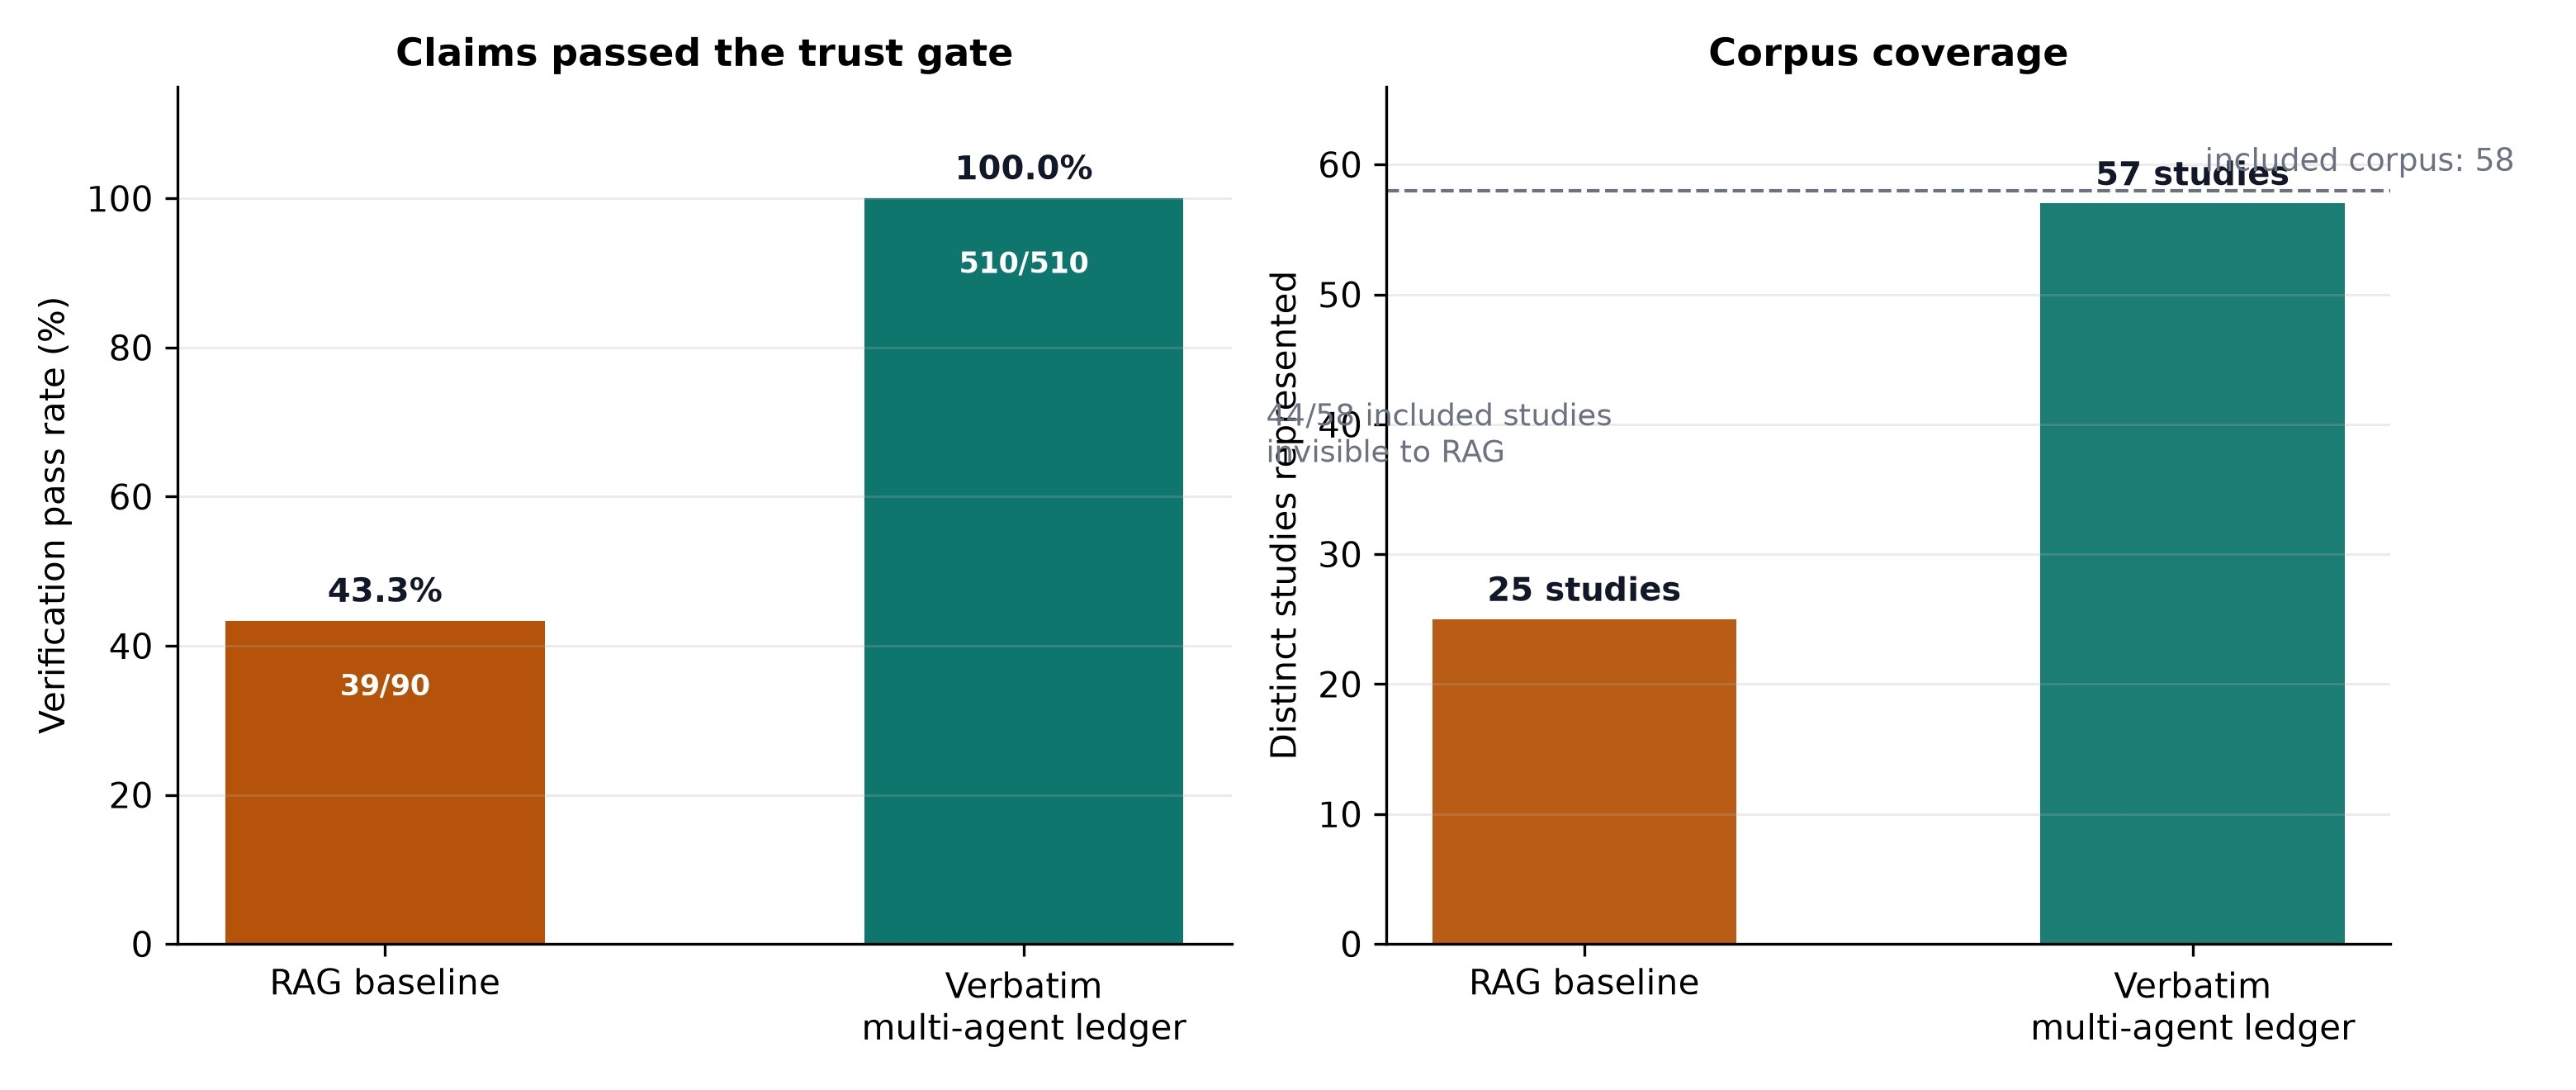
\includegraphics[keepaspectratio,alt={Figure 3 --- Head-to-head verification coverage: 43.3\% pass (39/90) and 25 studies represented for the RAG baseline versus 100\% (510/510) across 57/58 studies for the verbatim multi-agent ledger; 44/58 included studies invisible to RAG.}]{../../synthesis/figures_d2/fig1_verification_versus_coverage.png}}
\emph{Figure 3. Claim verification pass rate and corpus coverage,
Approach A vs.~B.}

\pandocbounded{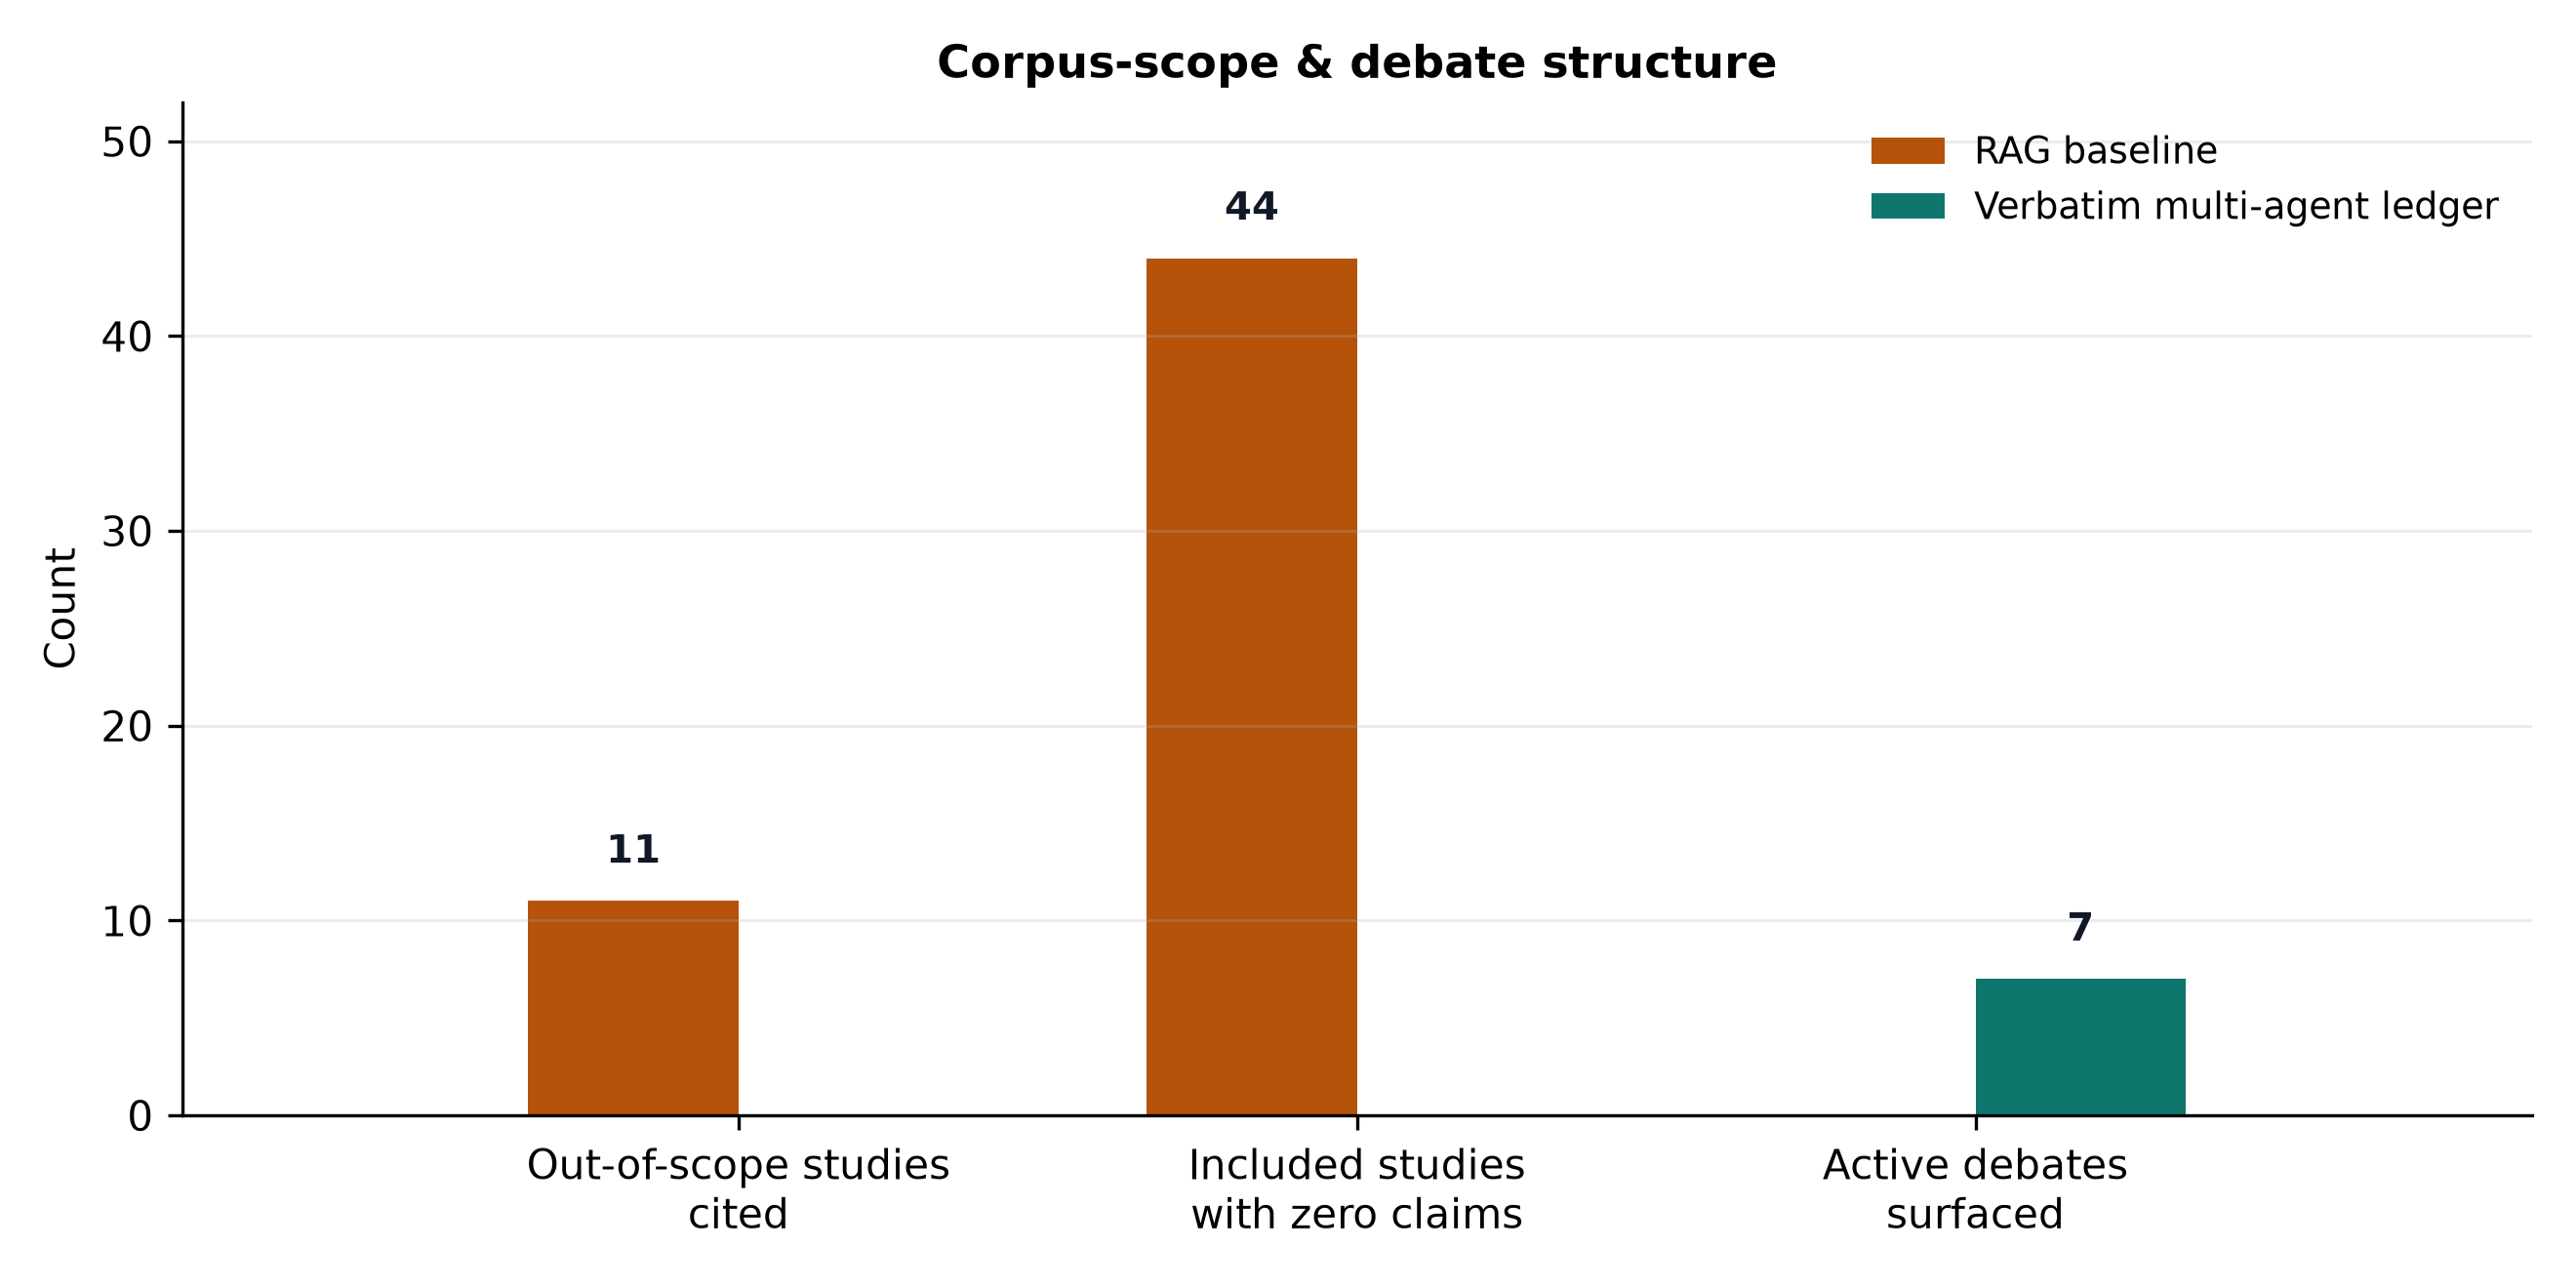
\includegraphics[keepaspectratio,alt={Figure 4 --- Corpus-scope discipline: RAG baseline cited 11 screened-out studies and left 44 included studies with zero claims; the verbatim ledger surfaced 7 active debates.}]{../../synthesis/figures_d2/fig2_scope_and_debates.png}}
\emph{Figure 4. Corpus-scope and debate structure (lower is better for
the first two panels; higher for debates).}

\pandocbounded{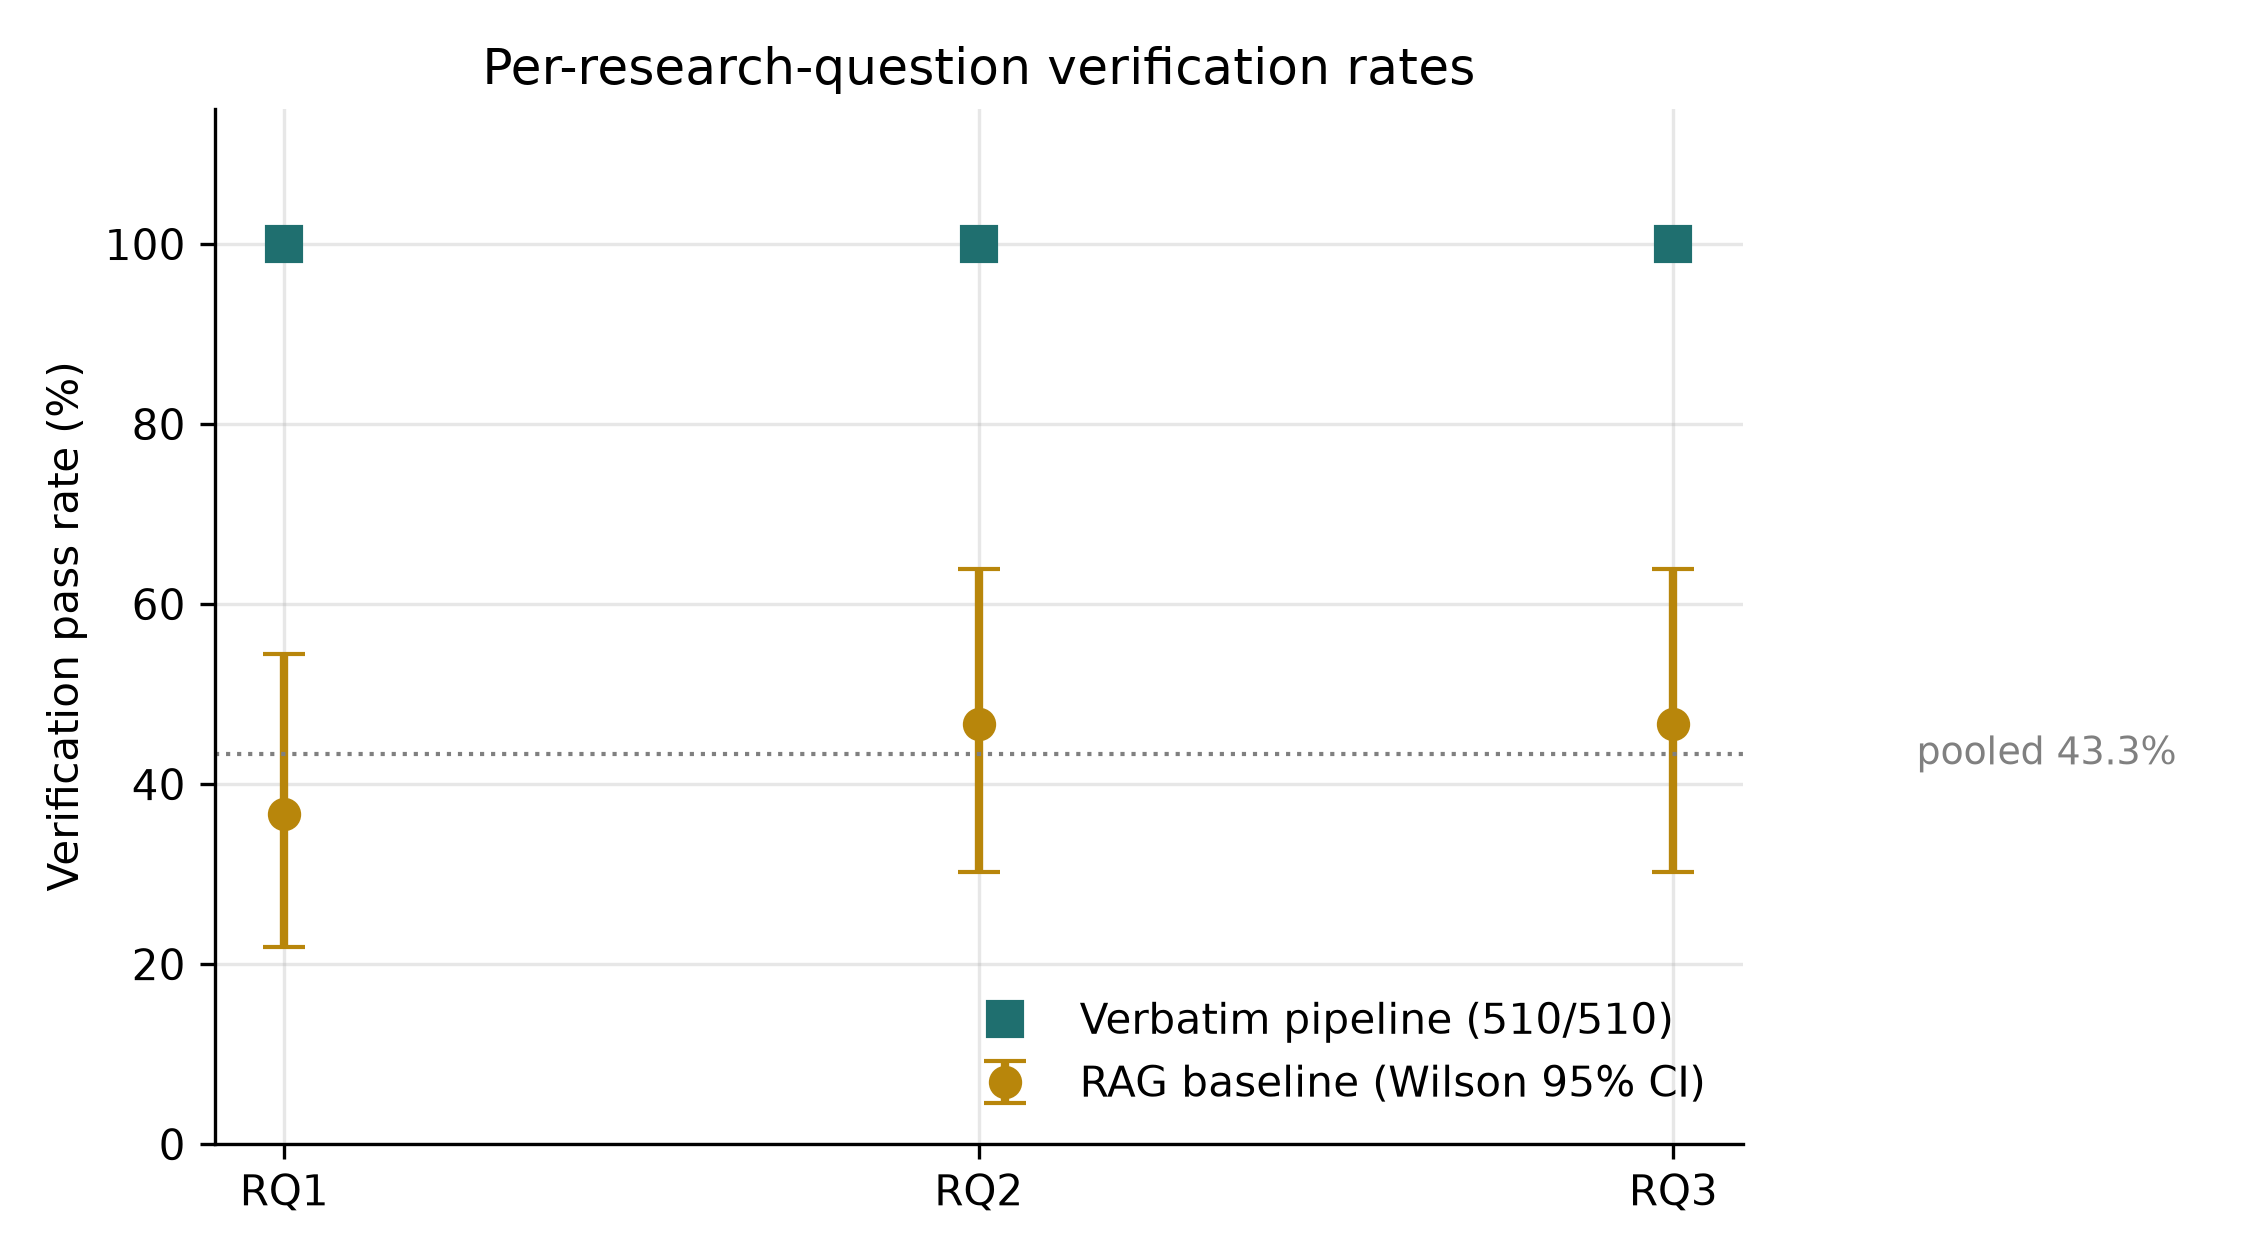
\includegraphics[keepaspectratio,alt={Figure 5 --- Per-research-question verification rates: RAG baseline 36.7\%/46.7\%/46.7\% (Wilson 95\% CIs) versus 100\% across RQ1--RQ3 for the verbatim ledger; pooled RAG floor 43.3\%.}]{../../synthesis/figures_d2/fig4_per_rq_rates.png}}
\emph{Figure 5. Per-research-question verification rates with 95\% CIs.}

\subsubsection{4.7 Phase-4 trust audit}\label{phase-4-trust-audit}

Retraction: 0/48 flagged. Open science: 16 repository links, 7 dual
data+code, 32 explicit DA/S/CA statements, 5 proprietary. COI: 5
industry ties (two Meta-affiliated, Google, Anthropic, OpenAI), 4
declared no-conflict, 1 academic-or-public, 37 with no formal COI
statement (of 47 scanned) --- a structural feature of computer-science
preprints and evocative of governance gaps the corpus itself describes.
Table 7 summarizes the four-stream audit.

\textbf{Table 7. Phase-4 trust-verification streams (Version 1.0).}

{\def\LTcaptype{none} % do not increment counter
\begin{longtable}[]{@{}
  >{\raggedright\arraybackslash}p{(\linewidth - 4\tabcolsep) * \real{0.3333}}
  >{\raggedright\arraybackslash}p{(\linewidth - 4\tabcolsep) * \real{0.3333}}
  >{\raggedright\arraybackslash}p{(\linewidth - 4\tabcolsep) * \real{0.3333}}@{}}
\toprule\noalign{}
\begin{minipage}[b]{\linewidth}\raggedright
Stream
\end{minipage} & \begin{minipage}[b]{\linewidth}\raggedright
Coverage
\end{minipage} & \begin{minipage}[b]{\linewidth}\raggedright
Finding
\end{minipage} \\
\midrule\noalign{}
\endhead
\bottomrule\noalign{}
\endlastfoot
Retraction status (OpenAlex/Crossref) & 48 studies checked & 0 flagged;
\texttt{crossref\_update\_events} empty (no supersession yet) \\
Open-science artifact scan (DA/S/CA) & 47 studies scanned & 16 repo
links · 7 dual data+code · 32 explicit statements · 5 proprietary \\
Conflict-of-interest audit & 47 studies scanned & 5 industry-equipment
ties · 4 declared no-conflict · 1 academic-or-public · 37 no formal
statement \\
Risk-of-bias attestation & 47 studies assessed &
PROBAST/QUADAS-2-adapted deterministic scoring \\
\end{longtable}
}

\subsection{5. Discussion}\label{discussion}

\subsubsection{5.1 Interpretation}\label{interpretation}

Three findings carry design consequences. \textbf{First}, provenance
engineering has matured into a concrete, implementable pattern language
--- structured logging, deterministic IDs, idempotency, content-hashed
commitments, open-weights selection, temperature-0 decoding --- that
converts ``traceability'' from a desideratum into a verifiable
mechanism, but adoption is uneven across the corpus. \textbf{Second},
citation verifiability is the binding trust constraint: over the corpus
observed, the 0.475 existence ceiling across 17,443 citations and the
discrepancy between retrieval-grounded (zero hallucinated papers) and
ungrounded (78--98\%) systems jointly imply that \textbf{non-grounded
claim generation is not defensible on current evidence} in this corpus,
and is a poor basis for scholarly infrastructure by our reading of the
included records. \textbf{Third}, evaluation practice lags the systems
it purports to assess: aggregate metrics (I² \textgreater{} 95\%,
domain-dependent AUC 0.77--0.95, item-level run instability,
semantic-similarity-proxy failures, −1.9\%/day drift) make single-number
validation claims unusable for trust certification.

\subsubsection{5.2 Implications for trustworthy research
infrastructure}\label{implications-for-trustworthy-research-infrastructure}

\begin{enumerate}
\def\labelenumi{\arabic{enumi}.}
\tightlist
\item
  \textbf{Append-only, file-based audit journals are the correct
  provenance primitive}, directly countering ephemeral logs and
  statistics that conceal item-level instability {[}8{]}{[}22{]}.
\item
  \textbf{Threshold-verified evidence is tractable and should be
  standard.} A full-text agent pipeline achieved 100\% pass at the
  stated ≥0.90 glyph-normalized coverage threshold on 510/510 claims;
  deterministic RAG reached 43.3\% on the same corpus.
\item
  \textbf{Corpus-scope discipline is mandatory.} Pre-screening
  extractions silently leak screened-out evidence into retrieval (11
  contaminated studies in the RAG baseline); synthesis must be confined
  to the reconciled included set.
\item
  \textbf{Trust verification precedes synthesis} --- retractions, COI
  ties, and open-science claims are knowable only through explicit
  Phase-4 streams.
\item
  \textbf{The field lacks its own benchmark.} Systems auditing review
  automation are themselves unaudited end-to-end; cross-domain,
  externally validated, jointly-evaluating infrastructure is the
  prerequisite for generalizable trust.
\end{enumerate}

\subsubsection{5.3 Limitations}\label{limitations}

Written tools were excluded from the review matrix to avoid
self-selection bias. Eleven included studies lack full text and
contribute the 17 abstract-only claims (12th included study has an empty
abstract and contributes none). \textbf{11 of 58 included studies could
not be Phase-4 certified} (absence of verifiable Crossref/OpenAlex
records at corpus finalization for the retraction stream and partial
metadata coverage for the other three streams; retraction stream covered
48) --- the attestation statistics in §4.7 use the study-scanned
denominators. The consensus clusterer uses a single embedding model and
a hand-set threshold (0.40). Verification at ≥0.90 coverage guarantees
that a quote matches its source at that threshold, not that the quote is
byte-identical or that the source is representative of its own corpus.
The corpus is preprint-track-heavy by design (55\% preprint, 52\% from
2026): this front-loads the newest evidence but makes aggregates
provisional and version-bound --- the living protocol (§3.8) absorbs
published-version supersession and subsequent runs rather than restating
finality. Screening agreement (κ = 0.408) is fair; screening decisions
were consensus-aggregated and adjudicated.

\subsection{6. Conclusion}\label{conclusion}

The 2023--2026 literature documents a rapid, convergent movement toward
auditable, provenance-bearing, retrieval- and agent-grounded research
harnesses --- and an equally rapid emergence of trust gaps (citation
fabrication ≤ 0.475 existence, item-level run instability,
semantic-proxy failures, absent benchmarks) that any credible
infrastructure must address. Our method --- protocol-driven scoping,
four-stream trust verification, threshold-verified full-text claim
extraction, and semantic consensus --- demonstrates, within this corpus,
that trustworthy agentic synthesis is achievable with currently
available tooling. The open research gap is a joint, externally
validated, multi-domain evaluation benchmark for the field.

\subsection{7. Declarations and Data
Availability}\label{declarations-and-data-availability}

\begin{itemize}
\tightlist
\item
  \textbf{Data availability}: full workspace
  \texttt{workspaces/ai-research-harnesses-trust/} (protocol, screening,
  extractions, claims ledger, consensus, audit journal, phase-4 outputs)
  is preserved and git-tracked (text/metadata) as versioned, hash-pinned
  artifacts. Supplementary: search-log per version
  (\texttt{literature/search\_log\_v1.0.json}), standalone flow of
  information (\texttt{synthesis/prisma\_scr\_flow.md} + vector figure
  \texttt{synthesis/figures/fig\_prisma\_scr\_flow.svg} and raster
  \texttt{fig\_prisma\_scr\_flow.png}), and reference-provenance map
  with preprint→published supersession tracking
  (\texttt{reports/supplementary\_references.md}).
\item
  \textbf{Code availability}: pipeline orchestration via Nexus Scholar
  kits; stage CLIs (\texttt{scholar-verify}
  retraction/open-science/coi/risk-of-bias + \texttt{verbatim-claims},
  \texttt{scholar-rag} index/consensus, discovery/screening entry
  points) are invocable in the project venv. Re-run instructions for the
  living-review protocol (§3.8): federated discovery and screening from
  \texttt{literature/}, extraction from \texttt{extracted/}, claim
  verification via the \texttt{scholar-verify\ verbatim-claims} gate
  (regeneration of the higher-level claim ledger uses the committed
  agent/prompt inputs recorded per run). Author-metadata resolution
  scripts for reference updates are committed under \texttt{scripts/}.
\item
  \textbf{Protocol availability}: hash-pinned protocol
  \texttt{protocol.json} (compiled-protocol fingerprint
  \texttt{sha256:9646d5ec6902c8f7687dfcb6568e473e1e01b78f666b20b74ec901f9703bf55c},
  recorded at last protocol recompile in the audit journal),
  \texttt{SCREENING\_CRITERIA.md}, and \texttt{intent.json}. Not
  externally registered at Version 1.0; registration is planned for a
  recognized registry (OSF) before journal submission.
\item
  \textbf{Preprints and updates}: this review explicitly includes
  preprint-track records (32/58). Preprint→published supersession is
  tracked where Crossref \texttt{update-to}/OpenAlex status is
  available; at Version 1.0 finalization these fields were empty for the
  corpus (see §5.3), so the living protocol (§3.8) is the mechanism by
  which supersession will be absorbed.
\item
  \textbf{Conflicts of interest}: none declared by the authors; the
  Nexus Scholar toolkit was excluded from the review matrix.
\item
  \textbf{Authors' contributions}: MB and SZ conceived and designed the
  review protocol, co-authored the manuscript, and jointly verified the
  evidence pipeline outputs; SZ provided supervision and methodological
  oversight; MB implemented the analyses.
\item
  \textbf{Funding}: this research received no specific grant from any
  funding agency in the public, commercial, or not-for-profit sectors.
\item
  \textbf{Traceability declaration}: every claim statistic in this
  manuscript is machine-verifiable against
  \texttt{synthesis/claims.json} (510 claims, each with verified
  evidence quotes) and \texttt{synthesis/consensus.json}; every pipeline
  step is recorded in \texttt{audit/journal.jsonl} (69 events). Version
  stamp: Review 1.0, corpus finalized 2026-09-09.
\end{itemize}

\begin{center}\rule{0.5\linewidth}{0.5pt}\end{center}

\subsection{References}\label{references}

{[}1{]} Islam MA. Designing a Human-AI Collaborative Modular Approach to
Automating Systematic Literature Reviews: From Objectives to Reporting.
Tampere University Institutional Repository. (2025).

{[}2{]} Paulraj NJ. Building an LLM Agent for Life Sciences Literature
QA and Summarization. World Journal of Advanced Research and Reviews.
(2025). doi: 10.30574/wjarr.2025.26.2.1665.

{[}3{]} Xie C, Kong W, Pi L, Qi D, Yang Y, Wang B, et al.~Performance of
Large Language Models in Automated Medical Literature Screening: A
Systematic Review and Meta‐Analysis. Journal of Evidence-Based Medicine.
(2026). doi: 10.1111/jebm.70166.

{[}4{]} Zhao C, Tang Y, Qian Y. Do Deployment Constraints Make LLMs
Hallucinate Citations? An Empirical Study across Four Models and Five
Prompting Regimes. arXiv. (2026). arXiv:2603.07287.

{[}5{]} Asai A, He J, Shao R, Shi W, Singh A, Chang JC, et
al.~Synthesizing scientific literature with retrieval-augmented language
models. Nature. (2026). doi: 10.1038/s41586-025-10072-4.

{[}6{]} Asai A, He J, Shao R, Shi W, Singh A, Chang JC, et
al.~OpenScholar: Synthesizing Scientific Literature with
Retrieval-augmented LMs. arXiv. (2024). doi: 10.48550/arxiv.2411.14199.
(preprint version of ref {[}5{]}. doi: 10.1038/s41586-025-10072-4)

{[}7{]} Kinas R, Krawczyk J, Powalski R, Pietrzak P, Kowalewska A,
Kolmus K, et al.~BioResearcher: Scenario-Guided Multi-Agent for
Translational Medicine. arXiv. (2026). arXiv:2605.05985.

{[}8{]} Figalová N, Huestegge L, Böckler-Raettig A. Evaluating human and
LLM screening workflows in a conceptually complex scoping review:
Recall--workload trade-offs and run-to-run consistency. arXiv. (2026).
arXiv:2608.26885.

{[}9{]} Susnjak T. Compiling Prompts, Not Crafting Them: A Reproducible
Workflow for AI-Assisted Evidence Synthesis. arXiv. (2025).
arXiv:2509.00038.

{[}10{]} Wysocki O, Wysocka M, Jacobo M, Unsworth H, Freitas A.
Biomedical reasoning in action: Multi-agent System for Auditable
Biomedical Evidence Synthesis. arXiv. (2025). doi:
10.48550/arxiv.2510.05335.

{[}11{]} Wang Z, Wei CH, Chan J, Leaman R, Day CP, Wu C, et
al.~DeepER-Med: Advancing Deep Evidence-Based Research in Medicine
Through Agentic AI. arXiv. (2026). arXiv:2604.15456.

{[}12{]} Huang YH, Lin YS. LUMEN: Cost-Transparent Multi-Agent Pipeline
for Automated Systematic Review and Meta-Analysis. arXiv. (2026).
arXiv:2606.28362.

{[}13{]} Taherinezhad M, Maier S, Vitagliano G, Pierri F, Feuerriegel S.
AutoSynthesis: An agentic system for automated meta-analysis. arXiv.
(2026). arXiv:2607.15247.

{[}14{]} Wang Z, Cao L, Danek B, Jin Q, Lu Z, Sun J. Accelerating
clinical evidence synthesis with large language models. npj Digital
Medicine. (2025). doi: 10.1038/s41746-025-01840-7.

{[}15{]} Lin HT, Yeh JT. meta-pipe: An LLM-agent pipeline for end-to-end
automated systematic review and meta-analysis. arXiv. (2026).
arXiv:2606.28363.

{[}16{]} Rouzrokh P, Khosravi B, Rouzrokh P, Shariatnia M. LatteReview:
A Multi-Agent Framework for Systematic Review Automation Using Large
Language Models. arXiv. (2025). doi: 10.48550/arxiv.2501.05468.

{[}17{]} Ha HH, Favre B, Portet F. MedMeta: A Benchmark for LLMs in
Synthesizing Meta-Analysis Conclusion from Medical Studies. arXiv.
(2026).

{[}18{]} Godinez A. HySemRAG: A Hybrid Semantic Retrieval-Augmented
Generation Framework for Automated Literature Synthesis and
Methodological Gap Analysis. arXiv. (2025). doi:
10.48550/arxiv.2508.05666.

{[}19{]} Rahgozar A, Mortezaagha P. AI Co-Scientist for Knowledge
Synthesis in Medical Contexts: A Proof of Concept. arXiv. (2026).
arXiv:2601.11825.

{[}20{]} Rahgozar A, Mortezaagha P, Edwards JD, Manuel DG, McGowen J,
Zwarenstein M, et al.~An AI-Driven Live Systematic Reviews in the
Brain-Heart Interconnectome: Minimizing Research Waste and Advancing
Evidence Synthesis. arXiv. (2025). doi: 10.48550/arxiv.2501.17181.

{[}21{]} Tongnamtiang S, Wongsim M, Satchawatee N. An AI-Assisted
Research Automation System for Scholarly Paper Retrieval and Review With
Workflow Orchestration. Journal of Computer Science. (2026). doi:
10.3844/jcssp.2026.2082.2091.

{[}22{]} Chen Z, Lu N, Li X, Ricard JA, Ju C, Wang HH, et al.~Bringing
analytic rigor to agentic AI for science: The Brain Researcher platform
for neuroimaging data analysis. arXiv. (2026). arXiv:2608.19902.

{[}23{]} Schmidt L, Hair K, Graziosi S, Campbell F, Kapp C, Khanteymoori
A, et al.~Exploring the use of a Large Language Model for data
extraction in systematic reviews: a rapid feasibility study. arXiv.
(2024). arXiv:2405.14445.

{[}24{]} Jaumann C, Wiedholz A, Friedrich A. LGAR: Zero-Shot LLM-Guided
Neural Ranking for Abstract Screening in Systematic Literature Reviews.
Findings of the Association for Computational Linguistics: ACL 2025.
(2025). doi: 10.18653/v1/2025.findings-acl.412.

{[}25{]} Serretti A. Benchmarking a Local Schema-Constrained Large
Language Model Pipeline for Abstract Screening and Evidence Mapping.
Cureus. (2026). doi: 10.7759/cureus.111193.

{[}26{]} Haryanto CY. LLAssist: Simple Tools for Automating Literature
Review Using Large Language Models. arXiv. (2024). doi:
10.48550/arxiv.2407.13993.

{[}27{]} Robinson A, Thorne W, Wu BP, Pandor A, Essat M, Stevenson M, et
al.~Bio-SIEVE: Exploring Instruction Tuning Large Language Models for
Systematic Review Automation. arXiv. (2023). doi:
10.48550/arxiv.2308.06610.

{[}28{]} Auer S, Oelen A, Jaradeh MY, Khalid M, Keya F, Gaddipati SK, et
al.~Towards AI-Supported Research: a Vision of the TIB AIssistant.
arXiv. (2025). arXiv:2512.16447.

{[}29{]} Matsumoto N, Choi H, Freda PJ, Hernandez ME, Wang ZP, Moore JH.
EcoXAI: Autonomous Agentic Ecosystem for Explainable Artificial
Intelligence and Biomedical Discovery. bioRxiv. (2026). doi:
10.64898/2026.07.08.737358.

{[}30{]} Zhang W, Nguyen T, Stuart EA, Chen YT. Large language models
for full-text methods assessment: a case study on mediation analysis.
Journal of the American Medical Informatics Association. (2026). doi:
10.1093/jamia/ocag108.

{[}31{]} Shafqat W, Patterson M, Liss SN. Knowledge Synthesis Review
Framework: Task-Level Benchmarking of LLM-Based Systems for Multi-Source
Evidence Synthesis. arXiv. (2026). arXiv:2608.12741.

{[}32{]} Zrubka M, Alexy M, György KT, Zrubka Z. Large Language Models
for Title/Abstract Screening in Systematic Literature Reviews: A Case
Study in Precision Livestock Farming. 2025 IEEE 25th International
Symposium on Computational Intelligence and Informatics (CINTI). (2025).
doi: 10.1109/cinti67731.2025.11311831.

{[}33{]} Moţăţăianu A, Păvăloiu IB. Advanced Semantic Analysis of
Research Papers Using a Retrieval-Augmented Architecture. Proceedings of
the International Conference on Business Excellence. (2026). doi:
10.2478/picbe-2026-0107.

{[}34{]} Ferreira Barros C, Kalinowski M, Kassab M, Neto VVG. On the Use
of a Large Language Model to Support the Conduction of a Systematic
Mapping Study: A Brief Report from a Practitioner's View. Proceedings of
the 2026 IEEE/ACM International Workshop on Methodological Issues with
Empirical Studies in Software Engineering. (2026). doi:
10.1145/3786149.3788298.

{[}35{]} Tang X, Duan X, Cai Z. Large Language Models for Automated
Literature Review: An Evaluation of Reference Generation, Abstract
Writing, and Review Composition. Proceedings of the 2025 Conference on
Empirical Methods in Natural Language Processing. (2025). doi:
10.18653/v1/2025.emnlp-main.83.

{[}36{]} Wang X, Zhang Y, Xu B, Hou L, Li J. DeepWeaver: Bridging the
Evidence Synthesis Gap in Open-Ended Question Answering. arXiv. (2026).
doi: 10.48550/arxiv.2608.18988.

\end{document}
